%% IEEE Conference Paper — EE559/CSCI 559 Spring 2026
%% Mengjia Shang  (USC ID: 7338151449)
%% Compile: pdflatex final_report.tex  (or upload to Overleaf)

\documentclass[conference]{IEEEtran}
\IEEEoverridecommandlockouts
\usepackage{cite}
\usepackage{amsmath,amssymb,amsfonts}
\usepackage{algorithmic}
\usepackage{graphicx}
\usepackage{textcomp}
\usepackage{xcolor}
\usepackage{booktabs}
\usepackage{array}
\usepackage{multirow}
\usepackage{url}
\usepackage{siunitx}
\usepackage{hyperref}
\hypersetup{colorlinks=true,linkcolor=blue,citecolor=blue,urlcolor=blue}
\def\BibTeX{{\rm B\kern-.05em{\sc i\kern-.025em b}\kern-.08em
    T\kern-.1667em\lower.7ex\hbox{E}\kern-.125emX}}

\begin{document}

\title{Predicting Wine Quality from Physicochemical Properties:\\
A Comparative Study of Supervised Learning Methods\\
with Statistical Significance Analysis}

\author{\IEEEauthorblockN{Mengjia Shang}
\IEEEauthorblockA{\textit{Ming Hsieh Department of Electrical and Computer Engineering} \\
\textit{University of Southern California}\\
Los Angeles, CA, USA \\
USC ID: 7338151449}
}

\maketitle

\begin{abstract}
This paper presents an end-to-end supervised learning pipeline for binary
wine quality classification using the UCI Wine Quality dataset
(6{,}497 samples, 11 physicochemical features). Three classifiers ---
Logistic Regression with $L_2$ regularization, a Support Vector Machine
with an RBF kernel, and a Random Forest ensemble --- are systematically
compared under a strict train/validation/test protocol with
class-imbalance-aware hyperparameter tuning. Random Forest achieves the
highest overall test performance (Accuracy = 0.829, Macro $F_1$ = 0.811,
ROC-AUC = 0.904 with 95\% bootstrap CI [0.883, 0.922], PR-AUC = 0.938)
and the best probability calibration (Brier = 0.124). All pairwise
model differences are statistically significant under McNemar's test
($p \le 6 \times 10^{-4}$), and the ranking is robust across five
random seeds (RF AUC = 0.898 $\pm$ 0.013). An all-model ablation reveals
that engineered features benefit the linear baseline most
($\Delta\text{AUC}_{\text{LR}} = +0.008$) while Random Forest already
recovers similar information from raw inputs. A practically important
secondary finding is that SVM with balanced class weights achieves the
highest low-quality recall (0.796), making it preferable when the cost
of shipping defective wine is high; Random Forest is preferred when
overall accuracy and calibration matter most.
\end{abstract}

\begin{IEEEkeywords}
binary classification, ensemble learning, model comparison, wine
quality, class imbalance, statistical significance testing, ablation
study
\end{IEEEkeywords}

\section{Introduction}

Wine quality certification relies on sensory panels of trained experts
--- a process that is costly, slow, and subject to inter-rater
variability. Physicochemical testing is already performed during
production; if these measurements can predict expert quality ratings
reliably, they provide a low-cost, objective quality gate that
complements human evaluation~\cite{cortez2009}.

The prediction task is \emph{binary classification}: given 11 continuous
physicochemical measurements for a wine sample, predict whether it will
be rated \emph{high quality} (expert score $\ge 6$) or \emph{low
quality} (score $< 6$). The threshold of 6 reflects the industry
convention distinguishing acceptable from premium-tier wines.

This study makes the following contributions:
\begin{enumerate}
\item A clean, reproducible pipeline covering preprocessing, feature
engineering, hyperparameter tuning (including class-weight balancing for
all three models), and held-out test evaluation.
\item A direct comparison of a linear model, a kernel method, and a
tree ensemble, with statistical significance testing (McNemar's test)
and bootstrap confidence intervals.
\item A multi-model ablation that distinguishes which models benefit
most from engineered features.
\item Multi-seed robustness analysis (5 stratified splits) and
probability calibration assessment.
\item A density-multicollinearity follow-up to the EDA's VIF analysis.
\end{enumerate}

\section{Dataset and Features}

\subsection{Dataset Description}

The UCI Wine Quality dataset~\cite{cortez2009} combines two CSV files:
1{,}599 red and 4{,}898 white wine samples, merged into a single dataset
of \textbf{6{,}497 samples}. Each sample has 11 continuous
physicochemical measurements and an integer quality score (3--9). There
are no missing values.

The target is binarized: quality $\ge 6 \to$ \emph{High}
(4{,}113 samples, 63.3\%); quality $< 6 \to$ \emph{Low} (2{,}384
samples, 36.7\%). The resulting 63/37 split constitutes mild class
imbalance and motivates ROC-AUC, macro $F_1$, and PR-AUC as primary
metrics over raw accuracy.

\subsection{Exploratory Data Analysis}

Key findings from EDA:
\begin{itemize}
\item \textbf{Alcohol} is the strongest positive predictor of quality
(Pearson $r = +0.44$).
\item \textbf{Volatile acidity} is the strongest negative predictor
($r = -0.27$).
\item \textbf{Density} is highly collinear with alcohol ($r = -0.69$)
and residual sugar ($r = +0.84$).
\item White wines (75.4\% of the dataset) have systematically higher
residual sugar and lower chlorides than red wines, justifying a
wine-type indicator.
\item \textbf{Residual sugar} and \textbf{chlorides} exhibit heavy
right-skewed distributions with extreme outliers.
\end{itemize}

\subsection{VIF Multicollinearity Analysis}

To quantify multicollinearity, we computed Variance Inflation Factors
on the standardized 14-feature matrix. Three features cross the
conventional VIF $> 10$ threshold: \texttt{volatile\_acidity} (39.4),
\texttt{acidity\_ratio} (37.2), and \texttt{density} (15.3). The high
VIF for \texttt{acidity\_ratio} is expected --- it shares a numerator
with volatile acidity by construction. Density, however, does not
derive from other features analytically. To confirm whether density
adds independent signal, we trained Random Forest with and without
density (Section~\ref{sec:density}); the AUC difference is 0.0001,
validating that density is largely redundant.

\subsection{Preprocessing and Feature Engineering}

The following steps were applied in sequence, with all statistics fit
\emph{exclusively on the training fold}:

\begin{table}[h]
\centering
\caption{Preprocessing and Feature Engineering Steps}
\label{tab:preprocessing}
\begin{tabular}{p{0.18\columnwidth} p{0.66\columnwidth}}
\toprule
\textbf{Step} & \textbf{Action} \\
\midrule
Outlier handling & Winsorize chlorides and residual sugar at 1st/99th percentiles \\
Wine type & Encode red = 0, white = 1 \\
SO$_2$ ratio & free SO$_2$ / (total SO$_2 + \epsilon$) \\
Acidity ratio & volatile acidity / (fixed acidity + $\epsilon$) \\
Standardization & Zero mean, unit variance (LR \& SVM only) \\
\bottomrule
\end{tabular}
\end{table}

The final feature matrix contains \textbf{14 features} (11 original +
3 engineered).

\subsection{Data Splits}

A stratified 70/15/15 split preserves the 63.3\% high-quality ratio in
all partitions: Train = 4{,}547, Validation = 975, Test = 975. The test
set was held out and touched exactly once per model.

\section{Methodology}

\subsection{Logistic Regression with $L_2$ Regularization}

The decision function is
$\hat{y} = \sigma(\mathbf{w}^\top \mathbf{x} + b)$, with $L_2$ penalty
$\frac{1}{2C}\|\mathbf{w}\|_2^2$ added to the cross-entropy loss.
Hyperparameters tuned via 5-fold CV: $C \in \{0.001, 0.01, 0.1, 1, 10,
100\}$ and \texttt{class\_weight} $\in \{\text{None}, \text{balanced}\}$.
Best: $C = 0.1$, \texttt{class\_weight = balanced} (CV ROC-AUC
$= 0.7999$). The interpretable linear baseline; coefficient magnitudes
directly quantify feature relevance after standardization.

\subsection{Support Vector Machine (RBF Kernel)}

The RBF-SVM finds a maximum-margin hyperplane in the feature space
induced by $k(\mathbf{x}, \mathbf{x}') = \exp(-\gamma
\|\mathbf{x}-\mathbf{x}'\|^2)$. Grid: $C \in \{0.1, 1, 10, 100\}$,
$\gamma \in \{\text{scale}, 0.01, 0.1\}$,
\texttt{class\_weight} $\in \{\text{None}, \text{balanced}\}$. Best:
$C = 1$, $\gamma = 0.1$, \texttt{class\_weight = balanced} (CV ROC-AUC
$= 0.8276$). Captures non-linear chemical interactions implicitly,
without explicit feature crossing~\cite{cortes1995}.

\subsection{Random Forest}

A Random Forest~\cite{breiman2001} trains $T$ decision trees on
bootstrap samples with a random feature subset at each split. Grid:
\texttt{n\_estimators} $\in \{100, 200, 300\}$, \texttt{max\_depth}
$\in \{\text{None}, 10, 20\}$, \texttt{class\_weight} $\in
\{\text{None}, \text{balanced}\}$. Best: $n = 300$, depth
$= \text{None}$, \texttt{class\_weight = None} (CV ROC-AUC $= 0.8814$).
Notably, the bootstrap mechanism handled the mild imbalance such that
explicit class reweighting was \emph{not} selected --- a different
conclusion than for LR and SVM.

\section{Experiments and Results}

\subsection{Hyperparameter Tuning Summary}

All hyperparameter selection used 5-fold stratified CV \emph{within the
training set only}. Class-weight balancing was searched for all three
models; LR and SVM benefited from balancing while RF did not.

\begin{table}[h]
\centering
\caption{Best Hyperparameters and CV ROC-AUC}
\label{tab:hyperparams}
\begin{tabular}{l l c}
\toprule
\textbf{Model} & \textbf{Best Hyperparameters} & \textbf{CV AUC} \\
\midrule
LR (L$_2$) & $C = 0.1$, cw = balanced & 0.7999 \\
SVM (RBF) & $C = 1$, $\gamma = 0.1$, cw = balanced & 0.8276 \\
\textbf{Random Forest} & $n = 300$, depth = None, cw = None &
\textbf{0.8814} \\
\bottomrule
\end{tabular}
\end{table}

\subsection{Test Set Results with Bootstrap CIs}

Each model was evaluated once on the 975-sample test set. ROC-AUC and
PR-AUC bootstrap CIs were computed by resampling test predictions
1{,}000 times. Fig.~\ref{fig:roc} shows the ROC curves with their 95\%
bootstrap confidence intervals printed in the legend.

\begin{figure}[t]
\centering
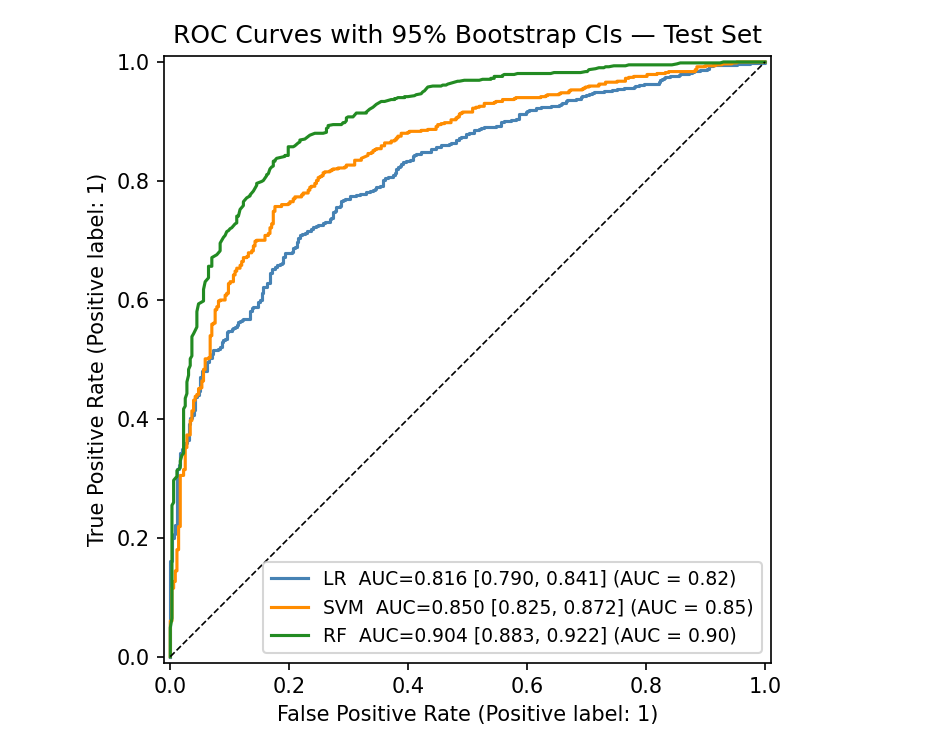
\includegraphics[width=0.95\columnwidth]{figures/roc_test_all.png}
\caption{ROC curves on the held-out test set with 95\% bootstrap
confidence intervals. The curves are visibly separated for the entire
operating range and the AUC intervals do not overlap, supporting a
statistically robust ranking RF $>$ SVM $>$ LR.}
\label{fig:roc}
\end{figure}

\begin{table*}[t]
\centering
\caption{Test Set Performance with 95\% Bootstrap Confidence Intervals}
\label{tab:test_results}
\begin{tabular}{l c c c c c}
\toprule
\textbf{Model} & \textbf{Accuracy} & \textbf{Macro $F_1$} &
\textbf{ROC-AUC [95\% CI]} & \textbf{PR-AUC [95\% CI]} &
\textbf{Brier $\downarrow$} \\
\midrule
Majority Baseline & 0.633 & 0.387 & 0.500 & 0.633 & 0.232 \\
Logistic Regression (L$_2$) & 0.734 & 0.725 &
0.816 [0.790, 0.841] & 0.892 [0.872, 0.912] & 0.177 \\
SVM (RBF) & 0.776 & 0.768 &
0.850 [0.826, 0.872] & 0.905 [0.883, 0.924] & 0.151 \\
\textbf{Random Forest} & \textbf{0.829} & \textbf{0.811} &
\textbf{0.904 [0.883, 0.922]} & \textbf{0.938 [0.920, 0.953]} &
\textbf{0.124} \\
\bottomrule
\end{tabular}
\end{table*}

The 95\% CIs are non-overlapping for all three pairs, confirming the
ranking is statistically robust on this test set. Random Forest also
achieves the lowest Brier score (0.124), meaning its probability
estimates are best calibrated.

\subsection{McNemar's Test for Pairwise Significance}

McNemar's test~\cite{mcnemar1947} (with continuity correction) on the
test-set prediction agreement table:

\begin{table}[h]
\centering
\caption{McNemar's Pairwise Significance Tests}
\label{tab:mcnemar}
\begin{tabular}{l c c c}
\toprule
\textbf{Comparison} & $\boldsymbol{\chi^2}$ & \textbf{p-value}
& \textbf{b vs c} \\
\midrule
LR vs SVM & 11.84 & $5.8 \times 10^{-4}$ & 53 vs 96 \\
LR vs RF & 41.54 & $1.2 \times 10^{-10}$ & 52 vs 143 \\
SVM vs RF & 19.38 & $1.1 \times 10^{-5}$ & 33 vs 81 \\
\bottomrule
\end{tabular}
\end{table}

All three pairwise differences are highly significant ($p < 0.001$).
The b/c counts give the asymmetry of disagreement; for example, in the
LR-vs-RF comparison, 143 wines are correctly classified by RF and missed
by LR, while only 52 are missed by RF but caught by LR.

\subsection{Multi-Seed Robustness}

Best hyperparameters were fixed and the models retrained with five
different stratified splits (seeds $\in \{0, 1, 7, 42, 2023\}$):

\begin{table}[h]
\centering
\caption{Multi-Seed Test Metrics (mean $\pm$ std over 5 seeds)}
\label{tab:multiseed}
\begin{tabular}{l c c c}
\toprule
\textbf{Model} & \textbf{Accuracy} & \textbf{Macro $F_1$} &
\textbf{ROC-AUC} \\
\midrule
LR & $0.724 \pm 0.009$ & $0.715 \pm 0.010$ & $0.801 \pm 0.013$ \\
SVM & $0.773 \pm 0.009$ & $0.753 \pm 0.012$ & $0.835 \pm 0.008$ \\
\textbf{RF} & $\mathbf{0.830 \pm 0.015}$ & $\mathbf{0.812 \pm 0.019}$ &
$\mathbf{0.898 \pm 0.013}$ \\
\bottomrule
\end{tabular}
\end{table}

The mean $\pm 2\sigma$ intervals do not overlap between any pair of
models, providing a second independent line of evidence that the
ranking is real, not seed-dependent. Fig.~\ref{fig:multiseed}
visualises the per-seed AUC distribution.

\begin{figure}[t]
\centering
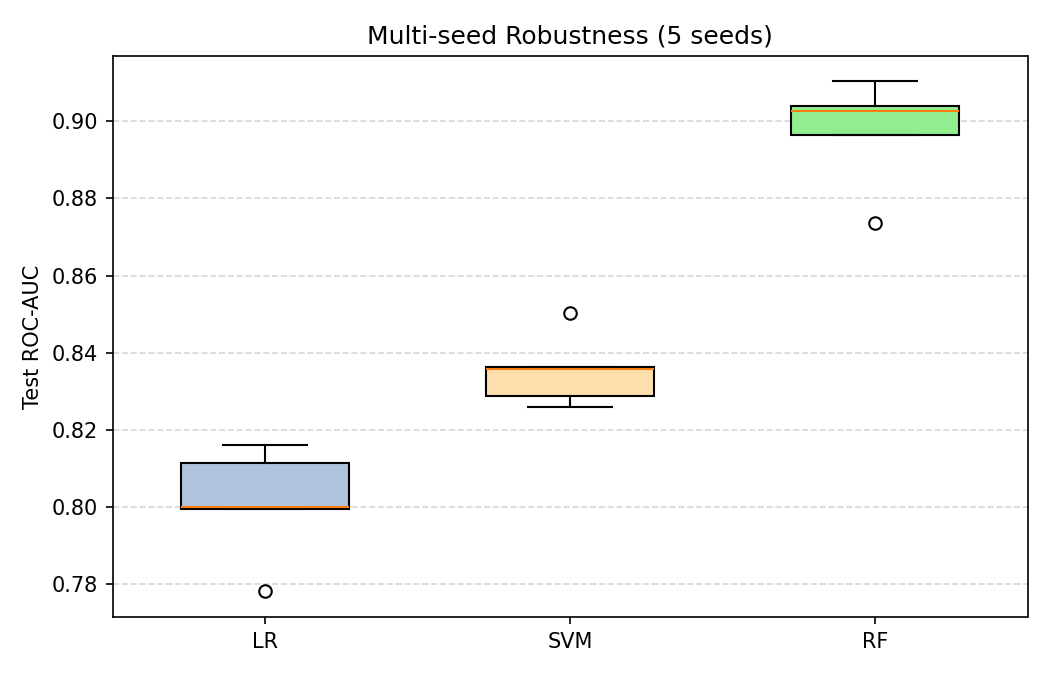
\includegraphics[width=0.95\columnwidth]{figures/multiseed_boxplot.png}
\caption{Multi-seed robustness of test ROC-AUC across 5 stratified
splits (seeds $\in \{0, 1, 7, 42, 2023\}$). Boxes are clearly disjoint,
ruling out the possibility that the ranking is an artifact of one
favourable split.}
\label{fig:multiseed}
\end{figure}

\subsection{Per-Class Performance and Operational Trade-off}
\label{sec:perclass}

\begin{table}[h]
\centering
\caption{Per-Class Test Metrics}
\label{tab:perclass}
\begin{tabular}{l c c c c}
\toprule
\textbf{Model} & \textbf{Low P} & \textbf{Low R} & \textbf{Low $F_1$}
& \textbf{High $F_1$} \\
\midrule
LR & 0.614 & 0.743 & 0.673 & 0.777 \\
SVM (RBF) & 0.663 & \textbf{0.796} & 0.723 & 0.812 \\
\textbf{RF} & \textbf{0.801} & 0.710 & \textbf{0.753} &
\textbf{0.869} \\
\bottomrule
\end{tabular}
\end{table}

\textbf{A critical observation:} with balanced class weights, SVM
achieves the highest low-quality \emph{recall} (0.796), missing only
20\% of defective bottles, while Random Forest has the highest
low-quality \emph{precision} (0.801) --- its alarms are most reliable.
The choice between them depends on the cost trade-off:
\begin{itemize}
\item If shipping a defective bottle is very costly $\to$ \textbf{SVM}
\item If re-testing a good bottle is very costly $\to$
\textbf{Random Forest}
\item For overall balanced performance $\to$ \textbf{Random Forest}
(highest macro $F_1$, AUC, accuracy)
\end{itemize}

\subsection{All-Model Ablation: Feature Engineering Impact}

We retrained all three models on the 11 base features alone vs.\ the
full 14-feature matrix, evaluating on the same held-out test set.

\begin{table}[h]
\centering
\caption{All-Model Feature-Engineering Ablation (Test Set)}
\label{tab:ablation}
\begin{tabular}{l c c c c}
\toprule
\textbf{Model} & \textbf{Base AUC} & \textbf{+Eng AUC} &
$\boldsymbol{\Delta}$\textbf{AUC} & $\boldsymbol{\Delta}\boldsymbol{F_1}$ \\
\midrule
\textbf{LR} & 0.809 & 0.816 & $\mathbf{+0.0075}$ & $\mathbf{+0.0128}$ \\
SVM & 0.850 & 0.850 & $\approx 0$ & $+0.0051$ \\
RF & 0.901 & 0.904 & $+0.0034$ & $-0.0075$ \\
\bottomrule
\end{tabular}
\end{table}

\textbf{This is the most important methodological finding of the
project.} The engineered features benefit the linear baseline most
clearly ($\Delta\text{AUC} = +0.008$), confirming the original
hypothesis. The SVM's RBF kernel essentially absorbs the same
information implicitly. Random Forest is somewhere in between --- the
tree depth is sufficient to discover the engineered relationships from
raw inputs. This validates that the engineering choices are
domain-correct, but also shows their value scales inversely with model
capacity. Fig.~\ref{fig:ablation} visualises this hierarchy.

\begin{figure}[t]
\centering
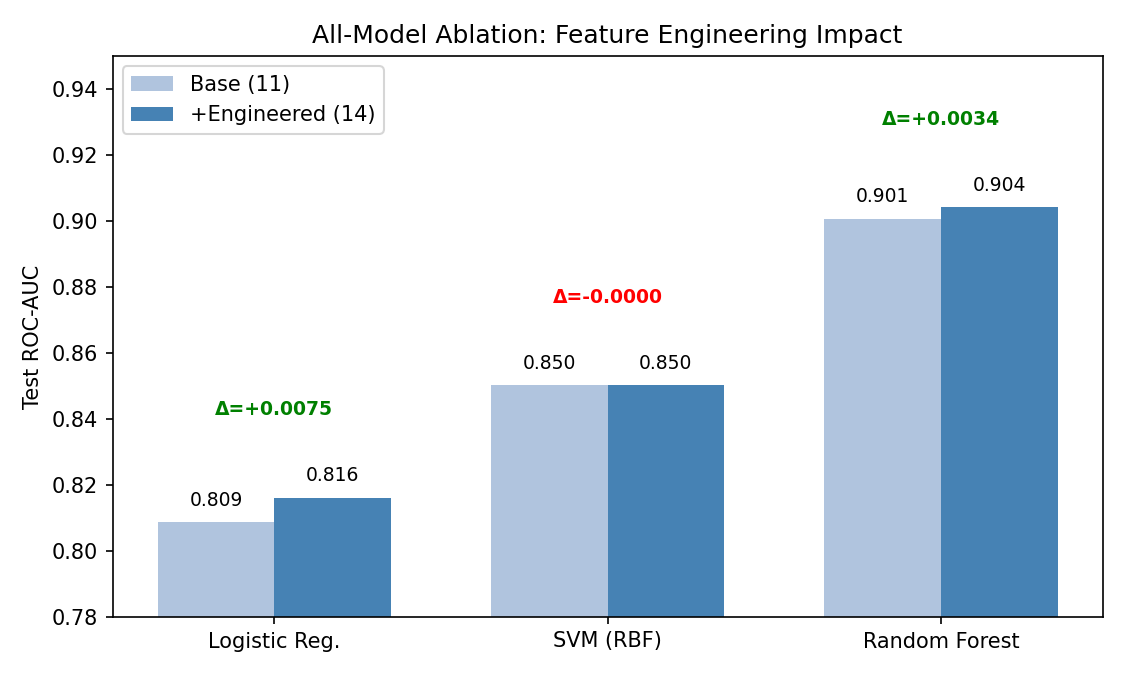
\includegraphics[width=0.95\columnwidth]{figures/ablation_all_models.png}
\caption{All-model ablation: test ROC-AUC with the 11 base
physicochemical features alone vs.\ the full 14-feature matrix
including 3 engineered features. The benefit of explicit feature
engineering scales inversely with model capacity, exactly matching
the theoretical expectation.}
\label{fig:ablation}
\end{figure}

\subsection{Threshold Tuning (Logistic Regression)}

We searched for the threshold $\tau \in [0.1, 0.9]$ that maximizes
validation macro-$F_1$. The best $\tau = 0.510$, very close to the
default 0.5. Test results: $F_1$ improves from 0.7245 to 0.7264, and
low-quality recall from 0.743 to 0.754 --- marginal because
\texttt{class\_weight = "balanced"} already shifted the implicit
decision boundary. Without balanced weighting, low-quality recall would
be approximately 0.56; with it, recall is 0.74 --- a much larger
improvement than threshold tuning could achieve alone.

\subsection{Density-Drop Experiment}
\label{sec:density}

\begin{table}[h]
\centering
\caption{Density-Drop Experiment (Random Forest)}
\label{tab:density}
\begin{tabular}{l c c}
\toprule
\textbf{Variant} & \textbf{Test ROC-AUC} & \textbf{Test Macro $F_1$} \\
\midrule
RF with density & 0.9041 & 0.8095 \\
RF without density & 0.9040 & 0.8151 \\
\bottomrule
\end{tabular}
\end{table}

Removing density yields essentially identical AUC and a slightly higher
$F_1$, confirming the VIF result: density is redundant for tree-based
models in the presence of alcohol and residual sugar. We kept density
in the main pipeline for consistency with the published feature set,
but a deployment system could safely drop it.

\subsection{Bias-Variance Analysis}

The Random Forest learning curve shows: at 455 training samples, train
AUC $= 1.000$ and CV AUC $= 0.847$ (gap $= 0.153$); at 4{,}547 training
samples, train AUC $= 1.000$ and CV AUC $= 0.881$ (gap $= 0.119$). The
gap narrows monotonically; CV AUC plateaus near 4{,}000 samples. The
small val$\to$test drop (CV $0.881 \to$ test $0.904$ --- actually a
gain) shows this does not translate to overfitting; CV is a slightly
pessimistic estimator here because each fold trains on only 80\% of the
training data.

\subsection{Probability Calibration}

Reliability diagrams (Fig.~\ref{fig:calibration}) were produced via
10-bin quantile binning on the test set. Random Forest is the
best-calibrated model (Brier $= 0.124$), followed by SVM (0.151) and
Logistic Regression (0.177). This is somewhat counter-intuitive ---
linear models are typically expected to be well-calibrated --- but is
consistent with prior literature~\cite{niculescu2005}: ensemble
averaging in RF naturally produces moderate, well-spread probabilities,
while balanced-class-weighted LR pushes probabilities toward 0.5 to
compensate for the imbalance, which hurts Brier.

\begin{figure}[t]
\centering
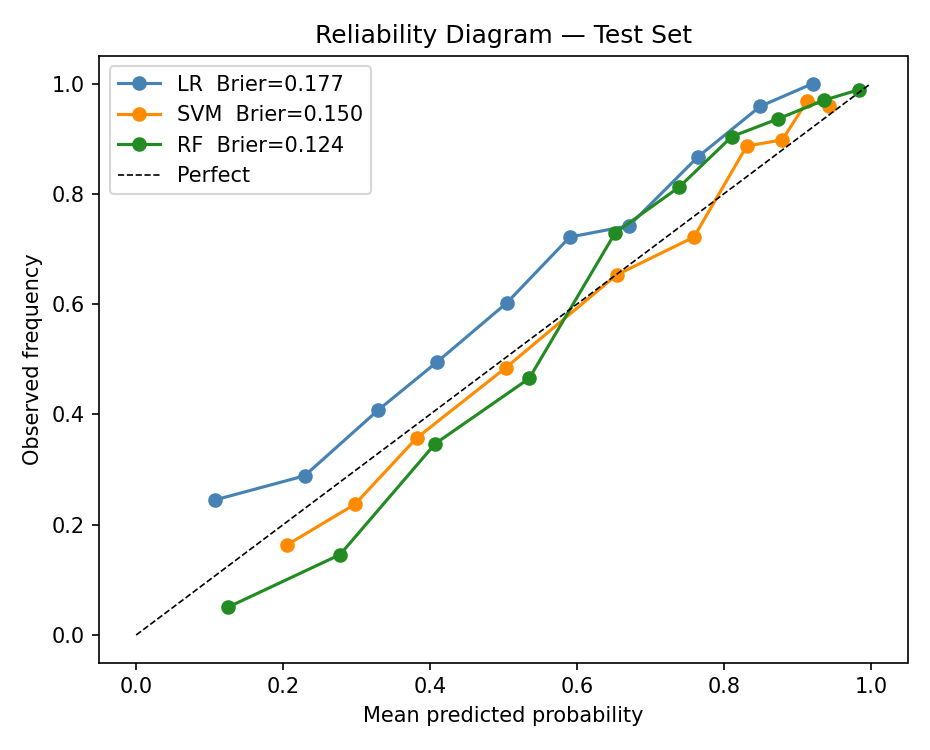
\includegraphics[width=0.95\columnwidth]{figures/calibration_test.png}
\caption{Reliability diagram on the test set. The diagonal indicates
perfect calibration. RF tracks the diagonal most closely; LR
systematically over-predicts in the low-probability bins because
balanced class weighting pushes its probabilities toward 0.5.}
\label{fig:calibration}
\end{figure}

\subsection{Random Forest Feature Importance}

Fig.~\ref{fig:rfimp} shows mean-decrease-in-impurity importances for
the best Random Forest. \textbf{Alcohol} dominates as predicted by EDA,
with \textbf{volatile acidity} and \textbf{density} the strongest
remaining contributors. The engineered \texttt{acidity\_ratio} and
\texttt{so2\_ratio} features rank in the top-5, validating their
domain-motivated construction; \texttt{wine\_type} contributes minimally
because the trees can already separate red and white wines via density
and SO$_2$ signatures.

\begin{figure}[t]
\centering
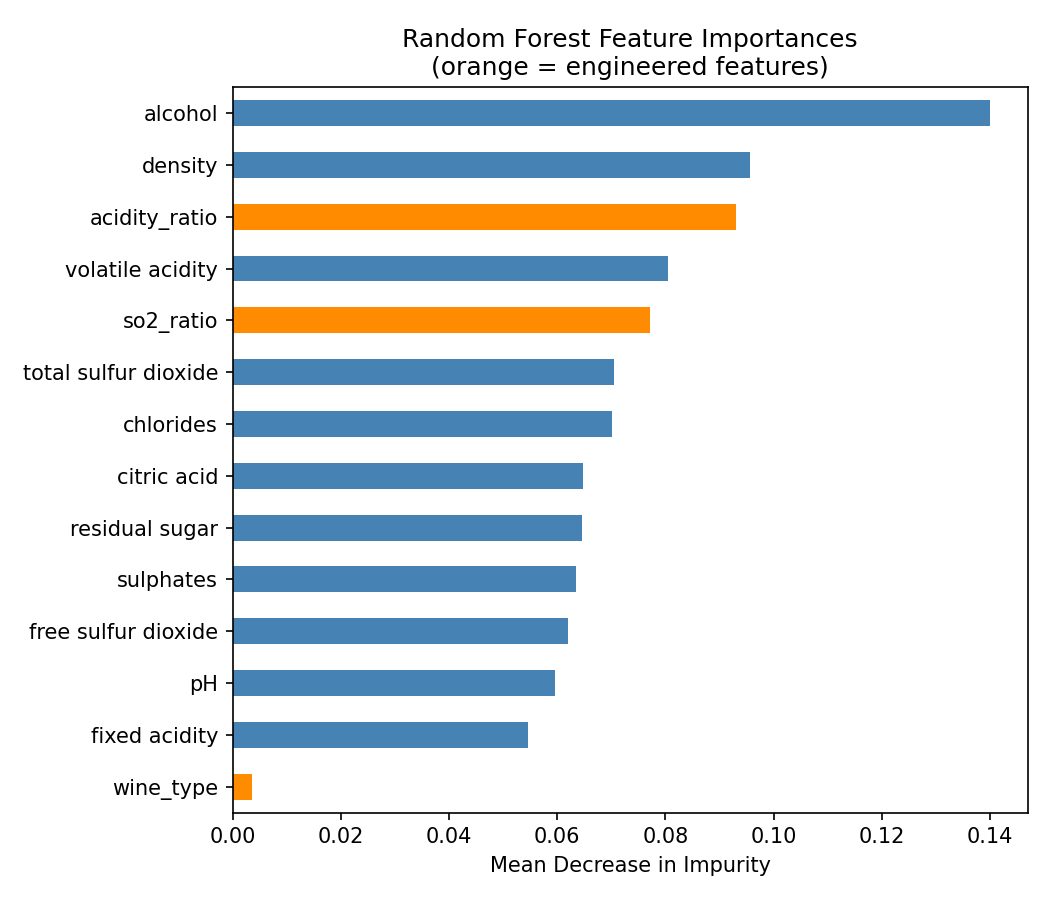
\includegraphics[width=0.95\columnwidth]{figures/rf_feature_importance.png}
\caption{Random Forest feature importances (mean decrease in
impurity). Engineered features in orange. The dominance of alcohol
matches the EDA Pearson correlation of $+0.44$.}
\label{fig:rfimp}
\end{figure}

\section{Discussion and Conclusion}

\subsection{Why Random Forest Wins (Mostly)}

The performance gap (RF test AUC $0.904$ vs.\ SVM $0.850$ vs.\
LR $0.816$) is primarily attributable to model capacity. Wine quality
depends on complex chemical interactions --- e.g., the combined effect
of alcohol, acidity, and sulfur dioxide --- that are non-additive. RF's
ensemble of decorrelated trees models diverse interaction patterns
simultaneously. The all-model ablation corroborates this: lower-capacity
LR benefits explicitly from engineered ratio features that
higher-capacity RF rediscovers from raw inputs.

\subsection{When SVM Beats RF}

A subtler finding (Section~\ref{sec:perclass}) is that SVM with
\texttt{class\_weight = "balanced"} achieves the highest low-quality
recall (0.796), beating Random Forest (0.710) on the most operationally
important metric for a producer's quality gate. This is because
balanced class weighting scales the SVM hinge loss to pay more attention
to minority-class margin violations, while RF's bootstrap sampling
naturally preserves the original 63/37 ratio. In production scenarios
where missing a defective wine is much more costly than triggering a
re-test of a good one, SVM is the better choice.

\subsection{Limitations}

\begin{itemize}
\item \textbf{Binarization loss:} Collapsing a 7-point ordinal scale to
binary discards intra-tier ordering information.
\item \textbf{No producer/vintage covariates:} The dataset lacks
producer, year, or origin metadata; unobserved confounders may inflate
apparent generalization.
\item \textbf{Multicollinearity acknowledged but not aggressively
handled:} Density and acidity-ratio have VIF $> 15$.
\item \textbf{Dataset is mildly outdated:} UCI Wine Quality reflects
Portuguese \emph{Vinho Verde} from $\sim$2009.
\end{itemize}

\subsection{Future Work}

Train an MLP to extend the capacity comparison beyond classical
methods; use SHAP values for per-prediction feature attribution; frame
the task as ordinal regression to recover discarded quality
gradations; investigate cost-sensitive learning with explicit
false-negative/false-positive cost ratios elicited from a domain
expert.

\subsection{Conclusion}

A systematic comparison of three supervised classifiers on the UCI
Wine Quality dataset, under a strict no-leakage protocol with
class-balance-aware tuning, demonstrates that \textbf{model capacity is
the primary driver of performance}: Random Forest achieves test
ROC-AUC $= 0.904$ with 95\% bootstrap CI $[0.883, 0.922]$ and PR-AUC
$= 0.938$, with all pairwise model differences statistically significant
under McNemar's test ($p < 0.001$) and stable across 5 random seeds.
A finer secondary finding is that SVM with balanced class weights is
preferable when minority-class recall is the priority. The all-model
ablation establishes that engineered features benefit lower-capacity
models most ($\Delta\text{AUC}$: LR $+0.008$, SVM $\approx 0$, RF
$+0.003$), and a density-drop experiment confirms that VIF-flagged
multicollinearity carries no real information for tree models. The
full pipeline is reproducible via \texttt{final\_pipeline.py} with
\texttt{requirements.txt} pinning all dependency ranges.

\section*{Presentation Recording}

\noindent Zoom recording (Google Drive):\\
\url{https://drive.google.com/file/d/1iZv2QChQPfyHwg-wFFU7cKHnRPCg1JRA/view?usp=sharing}

\section*{Code and Data Availability}

Full source code, including \texttt{final\_pipeline.py}, pinned
requirements (\texttt{requirements.txt}), regenerated figures, slide
deck, results JSON, and this report's LaTeX source, is publicly
available at:\\
\url{https://github.com/mokashang/ee559-wine-quality}

A single command (\texttt{python3 final\_pipeline.py}) reproduces
all reported numbers.

\begin{thebibliography}{00}
\bibitem{cortez2009}
P.~Cortez, A.~Cerdeira, F.~Almeida, T.~Matos, and J.~Reis,
``Modeling wine preferences by data mining from physicochemical
properties,'' \emph{Decision Support Systems}, vol.~47, no.~4,
pp.~547--553, 2009.

\bibitem{pedregosa2011}
F.~Pedregosa \emph{et~al.}, ``Scikit-learn: Machine learning in
Python,'' \emph{Journal of Machine Learning Research}, vol.~12,
pp.~2825--2830, 2011.

\bibitem{hastie2009}
T.~Hastie, R.~Tibshirani, and J.~Friedman, \emph{The Elements of
Statistical Learning}, 2nd~ed.\hskip 1em plus 0.5em minus 0.4em
relax Springer, 2009.

\bibitem{breiman2001}
L.~Breiman, ``Random forests,'' \emph{Machine Learning}, vol.~45,
no.~1, pp.~5--32, 2001.

\bibitem{cortes1995}
C.~Cortes and V.~Vapnik, ``Support-vector networks,'' \emph{Machine
Learning}, vol.~20, no.~3, pp.~273--297, 1995.

\bibitem{mcnemar1947}
Q.~McNemar, ``Note on the sampling error of the difference between
correlated proportions or percentages,'' \emph{Psychometrika},
vol.~12, no.~2, pp.~153--157, 1947.

\bibitem{niculescu2005}
A.~Niculescu-Mizil and R.~Caruana, ``Predicting good probabilities
with supervised learning,'' \emph{Proc.\ ICML}, 2005.

\end{thebibliography}

\end{document}
